\documentclass{report}
\usepackage[utf8]{inputenc}   % Encoding support
\usepackage{graphicx}         % To include images
\usepackage{listings}         % For code formatting
\usepackage{xcolor}           % To add colors
\usepackage{hyperref}         % For clickable links and references
\usepackage{amsmath, amssymb,amsthm} %For math
\usepackage{comment}
\usepackage{float}
\usepackage{minted}


\title{Report I}
\author{Kevin Deshayes}
\date{\2024-10-02}

\begin{document}

% ----- Title Page -----
\begin{titlepage}
    \centering
    {\huge\bfseries Report on Lab 1 \\[1cm]}  % Title
    \textbf{Author:} Kevin Deshayes\\[0.5cm]  % Author Name
    \textbf{Email:} kede23@student.bth.se\\[0.5cm]  % Email
    \textbf{Course Name:} Mathematical Statistics \\[0.5cm]  % Course Name
    \textbf{Course Code:} MS1403\\[1.5cm]  % Course Code
    
    \includegraphics[width=0.6\textwidth]{BTH_logo_gray.png} % Placeholder image
    \vfill
    \vspace{2cm}
\end{titlepage}

% ----- Table of Contents -----
\tableofcontents
\newpage
% ----- Code Example -----
\section{R code}



\begin{minted}[breaklines, linenos, frame=single, bgcolor=lightgray]{r}
#Assignment 1 MS1403
#Kevin Deshayes 
#kede23@student.bth.se
# Task 1: Implement three estimators and run experiments for different scenarios
n_values = c(10,20,50,90,140) #Global vector
# --- Define Estimators ---
# Estimator N1: Returns the maximum element in the sample
firstEstimator = function(n_values){
  #Will return the biggest element of the sample values
  return(max(n_values)); 
}
# Estimator N2: (n + 1) / n * Max(Sample)
secondEstimator = function(n_values){
  #do the (n+1/n)*firstEstimator(n_values) 
    n=length(n_values)
    x_n = max(n_values)
    N_2 = ( (n+1) / n) * x_n 
    return (N_2)
}
#For estimator N3
thirdEstimator = function(n_values){
    X_mean = mean(n_values)
    N_3 = 2*X_mean-1
    return(N_3) 
  }
# --- Main Experiment Function --- 
Experiment = function(N, n_values, repetitions = 5){
  ResultMean = data.frame(
    sample_size = n_values,
    Mean_Estimation1 = numeric(length(n_values)),  # Use lists to store multiple repetitions
    Mean_Estimation2 = numeric(length(n_values)),
    Mean_Estimation3 = numeric(length(n_values))
  )
  ResultVariance = data.frame(
    sample_size = n_values,
    Variance_Estimation1 = numeric(length(n_values)),
    Variance_Estimation2 = numeric(length(n_values)),
    Variance_Estimation3 = numeric(length(n_values))
  )
  #Iterate for 5 times
  for (n in n_values){
    #Store the estimations
    N1_reps = numeric(repetitions)
    N2_reps = numeric(repetitions)
    N3_reps = numeric(repetitions)
    for (i in 1:repetitions){
      #generate the result of the draws, size nrOF draws, results range from 1 to N
      #And stores them in the vector drawResult
      drawResult = sample(1:N, size = n, replace = TRUE, prob = NULL) 
      #Runs estimations using the drawResult and stores them in respective N_x container
      N1_reps[i] = firstEstimator(drawResult)
      N2_reps[i] = secondEstimator(drawResult)
      N3_reps[i] = thirdEstimator(drawResult)
    }
    # Find the row index that matches the current sample size
    row_index = which(ResultMean$sample_size == n)
    # Adds the mean estimation and variance for this n to results and rounds them to 5 digits, places it in the column for the current n
    ResultMean$Mean_Estimation1[row_index] = round(mean(N1_reps), digits = 5)
    ResultVariance$Variance_Estimation1[row_index] = round(var(N1_reps), digits = 5)
    ResultMean$Mean_Estimation2[row_index] = round(mean(N2_reps), digits = 5)
    ResultVariance$Variance_Estimation2[row_index] = round(var(N2_reps), digits = 5)
    ResultMean$Mean_Estimation3[row_index] = round(mean(N3_reps), digits = 5)
    ResultVariance$Variance_Estimation3[row_index] = round(var(N3_reps), digits = 5) 
  }
  #Combines the two data frames into a list of two data frames and returns that. 
    return(list(Means = ResultMean, Variances = ResultVariance)) 
}
# call the experiment function twice once for each scenario (Ns)
smallScenario = Experiment(30,n_values)
largeScenario = Experiment(150,n_values)
cat("For small scenario N=30", "\n")
cat("-------------------------------", "\n")
print(smallScenario$Means)
print(smallScenario$Variances)
cat("\n\n")
cat("For large scenario N=150", "\n")
cat("-------------------------------", "\n")
print(largeScenario$Means)
print(largeScenario$Variances)
\end{minted}

% ----- Results -----
\section{Results}
\begin{figure}[H]
    \centering
    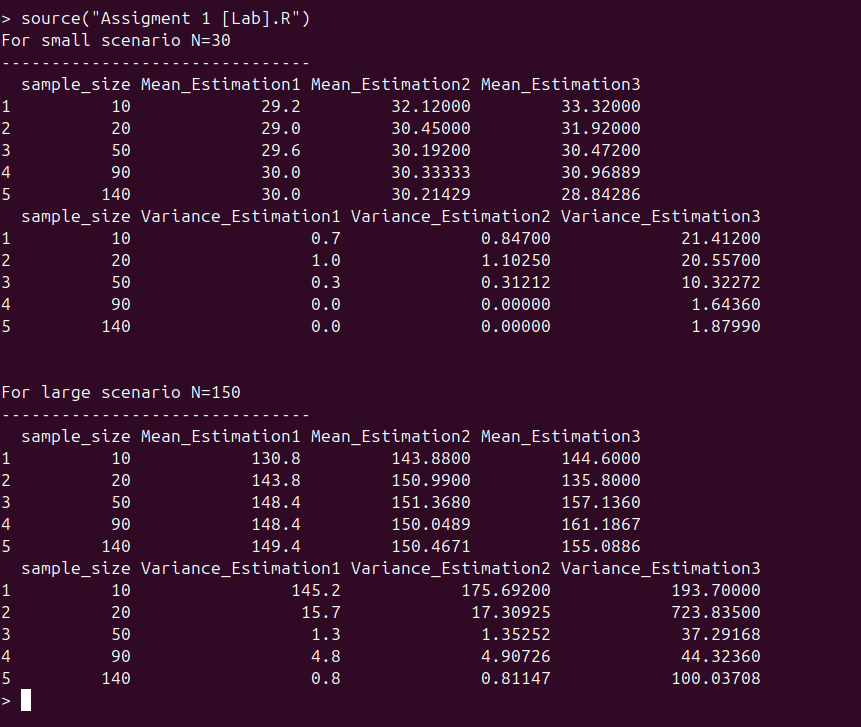
\includegraphics[width=1\linewidth]{OutputOfRCode.png}
    \caption{CLI output after running the code}
    \label{fig:enter-label}
\end{figure}


% ----- Data Analysis -----
\section{Analysis}

\subsection{Observations from the small scenario}


    $\hat{N}_2$ is most accurate overall with inaccuracy in smaller sample sizes. $\hat{N}_1$ is most accurate for smaller sample sizes and demonstrates higher consistency, with a marginally lower variance.$\hat{N}_3$ is relatively inaccurate with a high variance which leads to low consistency. 


\subsection{Observations from the large scenario}


    $\hat{N}_2$ is most accurate overall with inaccuracy in smaller sample sizes.$\hat{N}_1$ generally exhibits the lowest variance but has high inaccuracies for smaller sample sizes.$\hat{N}_3$ is relatively inaccurate with a high variance which leads to low consistency. 

\subsection{Discussion}

\begin{comment}
Figure 1 shows the mean estimations from the two experiments. The upper part of the figure for the small scenario and the lower part for the large scenario. It is observed that for all estimators, the variance decreases as the sample size increases, which aligns with the formula derived from the Central Limit Theorem. 
\end{comment}

In Figure 1, it is clear that all all estimators generally follow the Law of Large Numbers, where larger sample sizes tend to produce smaller variances, making the estimators more consistent and stable. However, there are still apparent spikes and deviations from this behavior. For example, in the large scenario, $\hat{N}_3$ variance jumps from 193 to 723 before eventually decreasing.

This can be explained by the sensitivity of the estimator to outliers or inherent instability when working with random sampling. The high variance of 723 demonstrates how unstable $\hat{N}_3$ can be when dealing with extreme values in the sample. This result is not an anomaly but highlights the nature of $\hat{N}_3$. The reason is that $\hat{N}_3$ is based on the sample mean, which is highly susceptible to outliers or extreme values, especially for small sample sizes.

To address this, increasing the sample size and the number of repetitions would help stabilize the variance for all estimators, but especially for $\hat{N}_3$.


\subsection{Conclusions}

\begin{itemize}
    \item $\hat{N}_1$: Best suited for smaller N values. Consistent with low variance. 
    \item $\hat{N}_2$: The most accurate estimator in both small and large scenarios.
    \item $\hat{N}_3$: Highly unstable, particularly with small sample sizes, due to its reliance on the sample mean, which is prone to large variances from extreme values.
    \item Law of Large Numbers: Observed in general trends, but temporary spikes can still occur, especially in $\hat{N}_3$ due to sensitivity to random fluctuations.
\end{itemize}

\end{document}
